\vspace{0.2cm}
\subsection{Design and Manufacturing Process}

\subsubsection{Conceptual Design}

The design process began with a comprehensive evaluation of last year’s ROV to identify areas for improvement. The team focused on two primary aspects: performance optimization and the integration of new features required for this year’s tasks.

To ensure a structured approach, brainstorming meetings were conducted to analyze feasibility, cost, and impact on overall performance. One of the major innovations was the adoption of a modular aluminum extrusion body, a strategic decision aimed at enhancing adaptability and extending the ROV’s lifespan. 

\hspace{10pt} Another key challenge was selecting suitable material for the electronic canister. An aluminum design was initially considered but was found to be twice as expensive as a 3D-printed alternative. After evaluating material strength and pressure resistance, the team decided to proceed with 3D printing, ensuring a cost-effective and flexible solution that could withstand underwater conditions while being easy to assemble and modify.

\subsubsection{Preliminary Design}

Once the core design concepts were defined, SolidWorks simulations were conducted to evaluate structural integrity, hydrodynamics, and thruster configurations. These data-driven insights played a critical role in optimizing component placement and material selection.

\hspace{10pt} To ensure an optimal balance between performance and affordability, a trade-off matrix (Table \ref{tab:material_selection}) was developed, comparing materials based on weight, cost, and manufacturability. The table presents the weighted selection criteria per component according to  a weighted sum presented in Equation \ref{eq:material_selection}, where materials are chosen by maximizing the sum of weighted property scores. Additionally, build vs. buy decisions were assessed, ensuring that in-house manufacturing was pursued where it provided a functional and economic advantage, while outsourcing was considered for components requiring specialized fabrication.

\scriptsize
\begin{equation}
  \label{eq:material_selection}
  \text{Total Score} = \sum_{\textit{Criteria}=1}^{n} (\text{component weight})_{\textit{criteria}} \times (\text{material score})_{\textit{criteria}}
\end{equation}
\normalsize

\begin{table}[h]
  \centering
  \renewcommand{\arraystretch}{1.2} 
  \begin{adjustbox}{width=\columnwidth}
  \begin{tabular}{|cc|cccc|ccccc|c|}
  \hline
  \multicolumn{2}{|c|}{\multirow{2}{*}{\textbf{Criteria}}} & \multicolumn{4}{c|}{\textbf{Weight}} & \multicolumn{5}{c|}{\textbf{Materials}} & \multirow{2}{*}{Selected Material} \\ \cline{3-11}
  & & Frame & Body & Canister & Gripper & HDPE & Acrylic & Aluminum & Stainless steel & 3D printing & \\ \hline
  \multicolumn{1}{|c|}{1} & Transparency & 0 & 0 & 0.1 & 0 & 0 & 10 & 0 & 0 & 0 & - \\
  \multicolumn{1}{|c|}{2} & Strength & 0.1 & 0.4 & 0.3 & 0.2 & 6 & 4 & 9 & 10 & 6 & - \\
  \multicolumn{1}{|c|}{3} & Cost \& Availability & 0.2 & 0.2 & 0.3 & 0.4 & 8 & 6 & 7 & 5 & 8 & - \\
  \multicolumn{1}{|c|}{4} & Fabrication (ease) & 0.5 & 0.3 & 0.2 & 0.2 & 9 & 7 & 7 & 6 & 8 & - \\
  \multicolumn{1}{|c|}{5} & Ductility & 0.1 & 0.1 & 0.1 & 0.1 & 7 & 3 & 8 & 6 & 4 & - \\
  \multicolumn{1}{|c|}{6} & Specific Gravity & 0.1 & 0 & 0 & 0.1 & 9 & 8 & 7 & 2 & 8 & - \\ \hline
  \multicolumn{2}{|c|}{\multirow{4}{*}{\textbf{Total Score}}} & \multicolumn{4}{c|}{Frame} & \textbf{8.3} & 6.5 & 7.3 & 4.6 & 7.4 & HDPE \\
  & & \multicolumn{4}{c|}{Body} & 7.7 & 5.6 & \textbf{8.1} & 6.8 & 7 & Aluminum \\
  & & \multicolumn{4}{c|}{Canister} & 7.1 & 5.3 & 6.8 & 4.7 & \textbf{7.5} & 3D Printing \\
  & & \multicolumn{4}{c|}{Gripper} & \textbf{7.6} & 5.2 & 6.8 & 5.6 & 7.4 & HDPE \\ \hline
  \end{tabular}
  \end{adjustbox}
  \caption{Criteria and Material Selection Matrix.}
  \label{tab:material_selection}
  
\end{table}

\hspace{10pt} To validate these theoretical analyses, small-scale prototypes were developed for key components. The 3D-printed canister was tested for sealing effectiveness, and successful trials confirmed its reliability before moving to full-scale manufacturing. Camera housings were also prototyped to optimize field-of-view placement. This iterative process allowed for practical verification of design choices before finalizing the ROV.

\subsubsection{Detailed Design and Manufacturing}

With validated designs, the final ROV model (Figure \ref{fig:kamikaze_drawings}) was fully developed in SolidWorks, incorporating stress, buoyancy, and flow simulations to ensure structural stability and hydrodynamic efficiency.

\begin{figure}[h]
    \centering
    \rule{0.8\columnwidth}{4cm}
    \caption{Kamikaze Drawings}
    \label{fig:kamikaze_drawings}
\end{figure}

For manufacturing, a systems-based approach was taken:

\vspace{-0.5\baselineskip}
\begin{itemize}
    \setlength{\itemsep}{0pt}
    \item The aluminum plates body was Laser CNC-machined and assembled using precise modular connectors.
    \item The canister was made using 3D printing, with design improvements tested through simulation and prototype experiments.
    \item The grippers and other HDPE parts were cut using router cutters, leveraging precise CAD models to minimize material waste. 2D CAD models (Figure \ref{fig:dxf}) were generated to optimize material usage.
\end{itemize}

\begin{figure}[h]
    \centering
    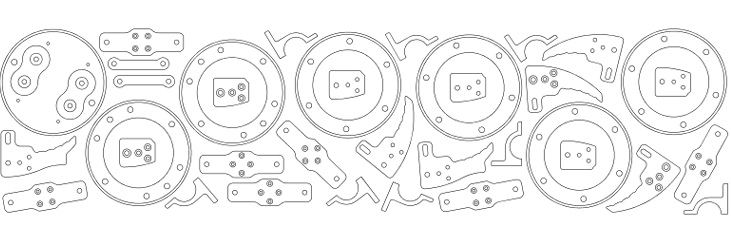
\includegraphics[width=0.8\columnwidth]{Sections/2Design Rationale/images/DXF.png}
    \caption{DXF file for cutting the float and grippers.}
    \label{fig:dxf}
\end{figure}

For the electrical system, significant innovations were implemented:

\vspace{-0.5\baselineskip}
\begin{itemize}
    \setlength{\itemsep}{0pt}
    \item The ESCs were integrated into a single PCB, reducing wiring complexity, electrical noise, and space consumption within the canister. This improvement streamlined system integration and enhanced overall performance. (Figure \ref{fig:pcb})
    \item A custom-designed depth sensor replaced the previous board, offering higher accuracy, real-time measurements, and expanded connectivity options. This upgrade ensured more precise and reliable depth control.
\end{itemize}

\begin{figure}[h]
    \centering
    \begin{subfigure}{0.4\columnwidth}
      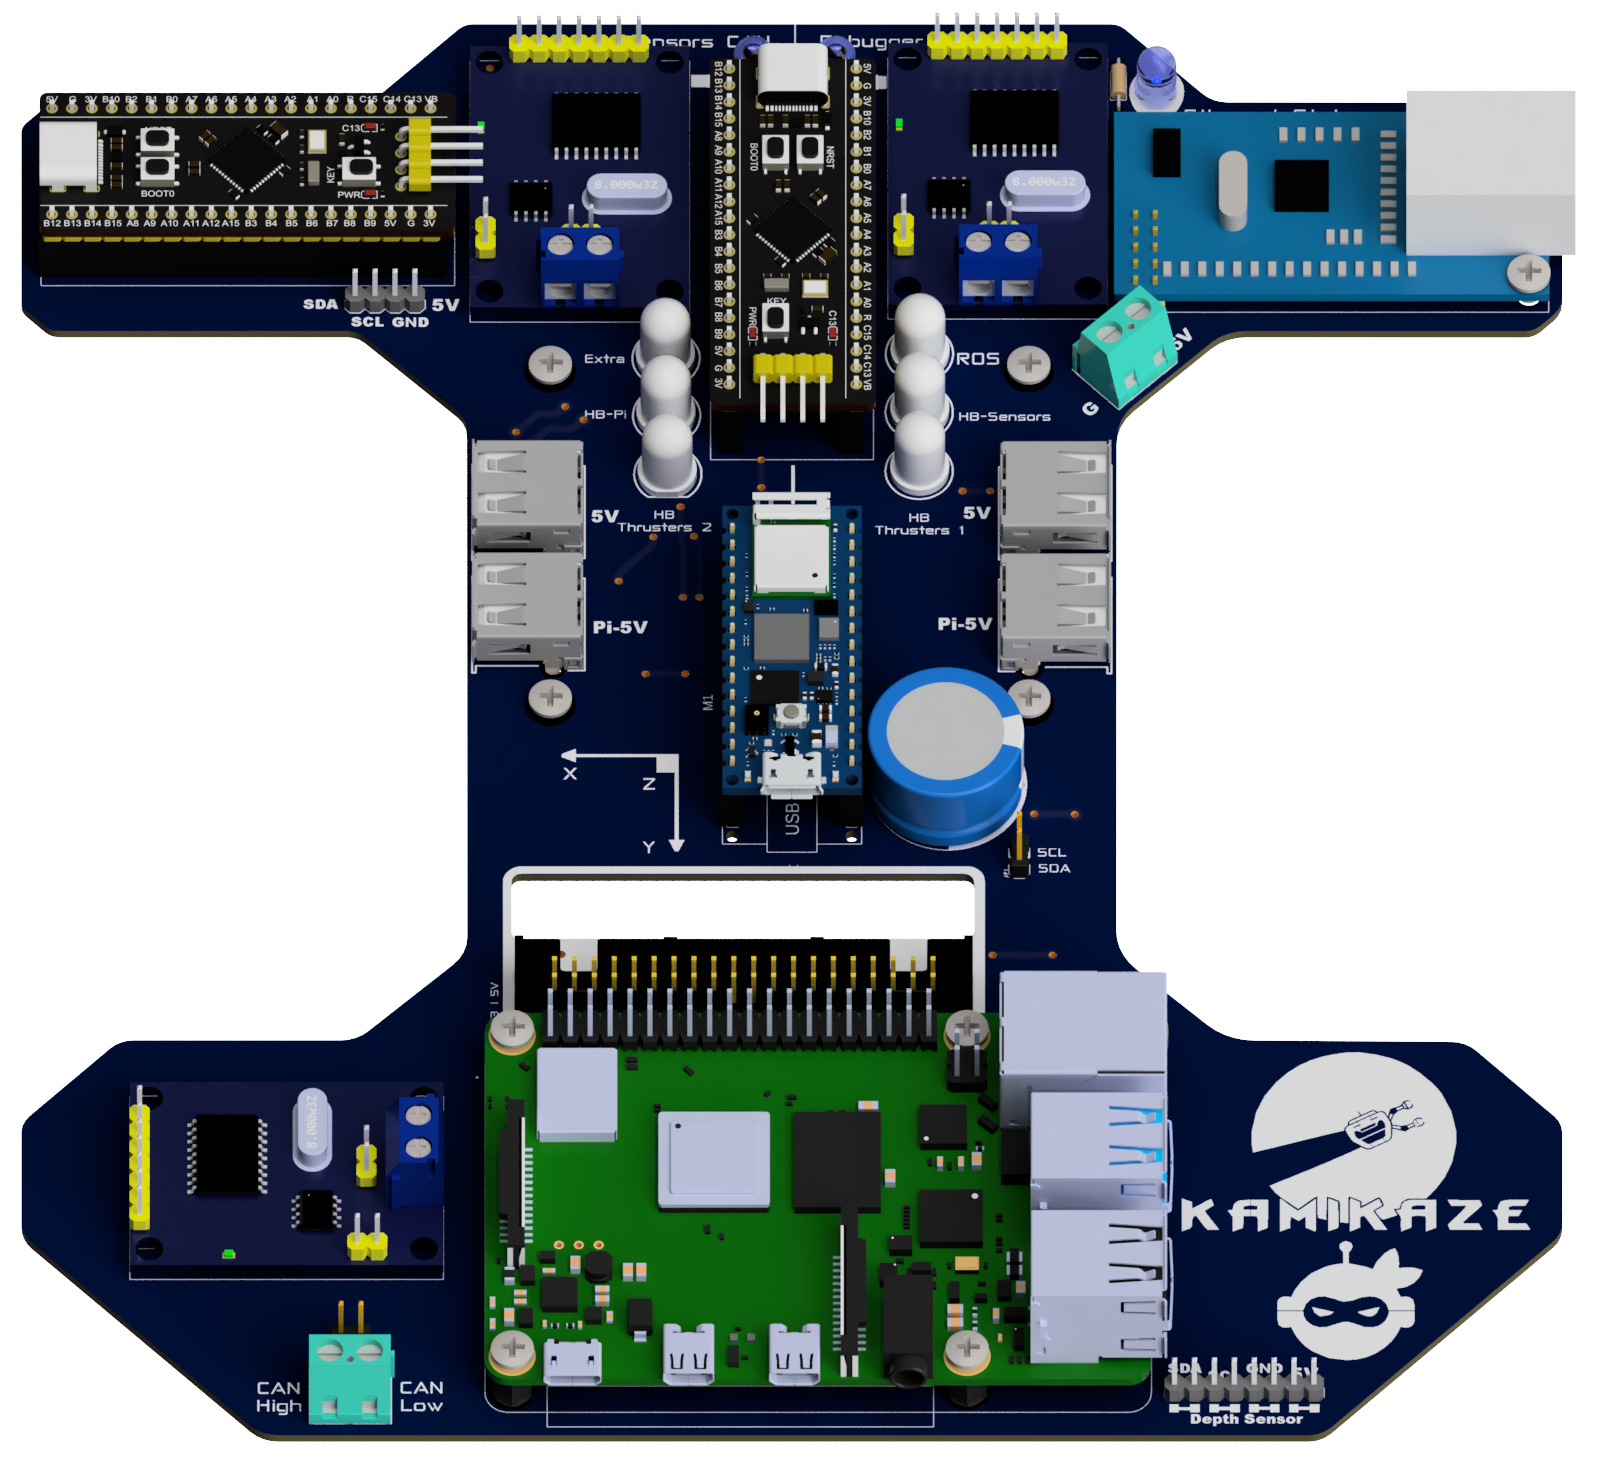
\includegraphics[width=\textwidth]{Sections/2Design Rationale/images/Control PCB.png}
      \caption{Control PCB.}
    \end{subfigure}
    \hfill
    \begin{subfigure}{0.15\columnwidth}
      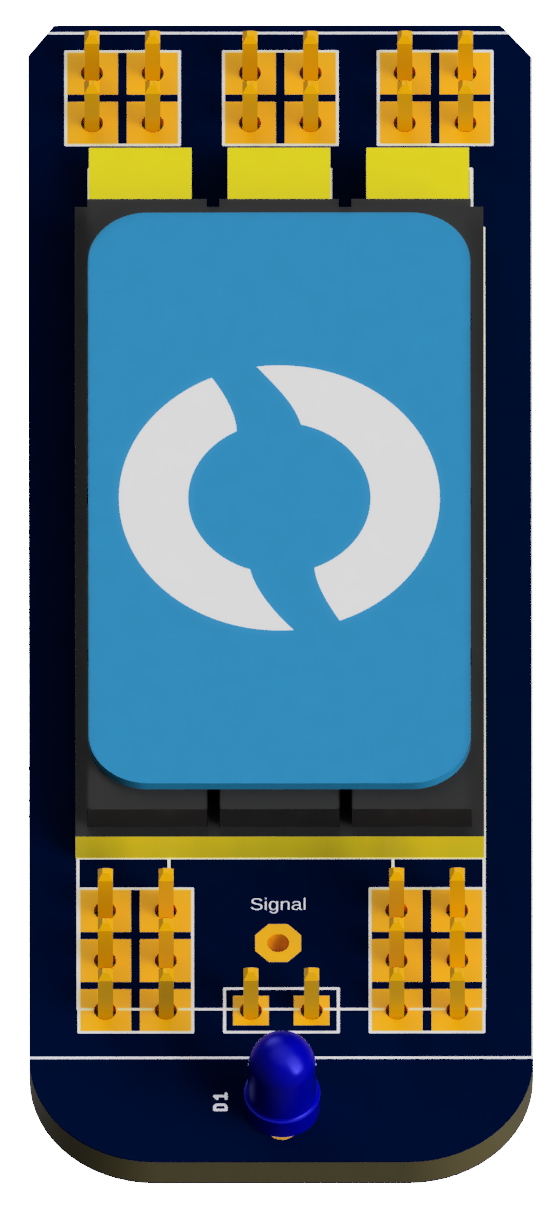
\includegraphics[width=\textwidth]{Sections/2Design Rationale/images/ESC PCB.png}
      \caption{ESC PCB.}
    \end{subfigure}
    \hfill
    \begin{subfigure}{0.4\columnwidth}
      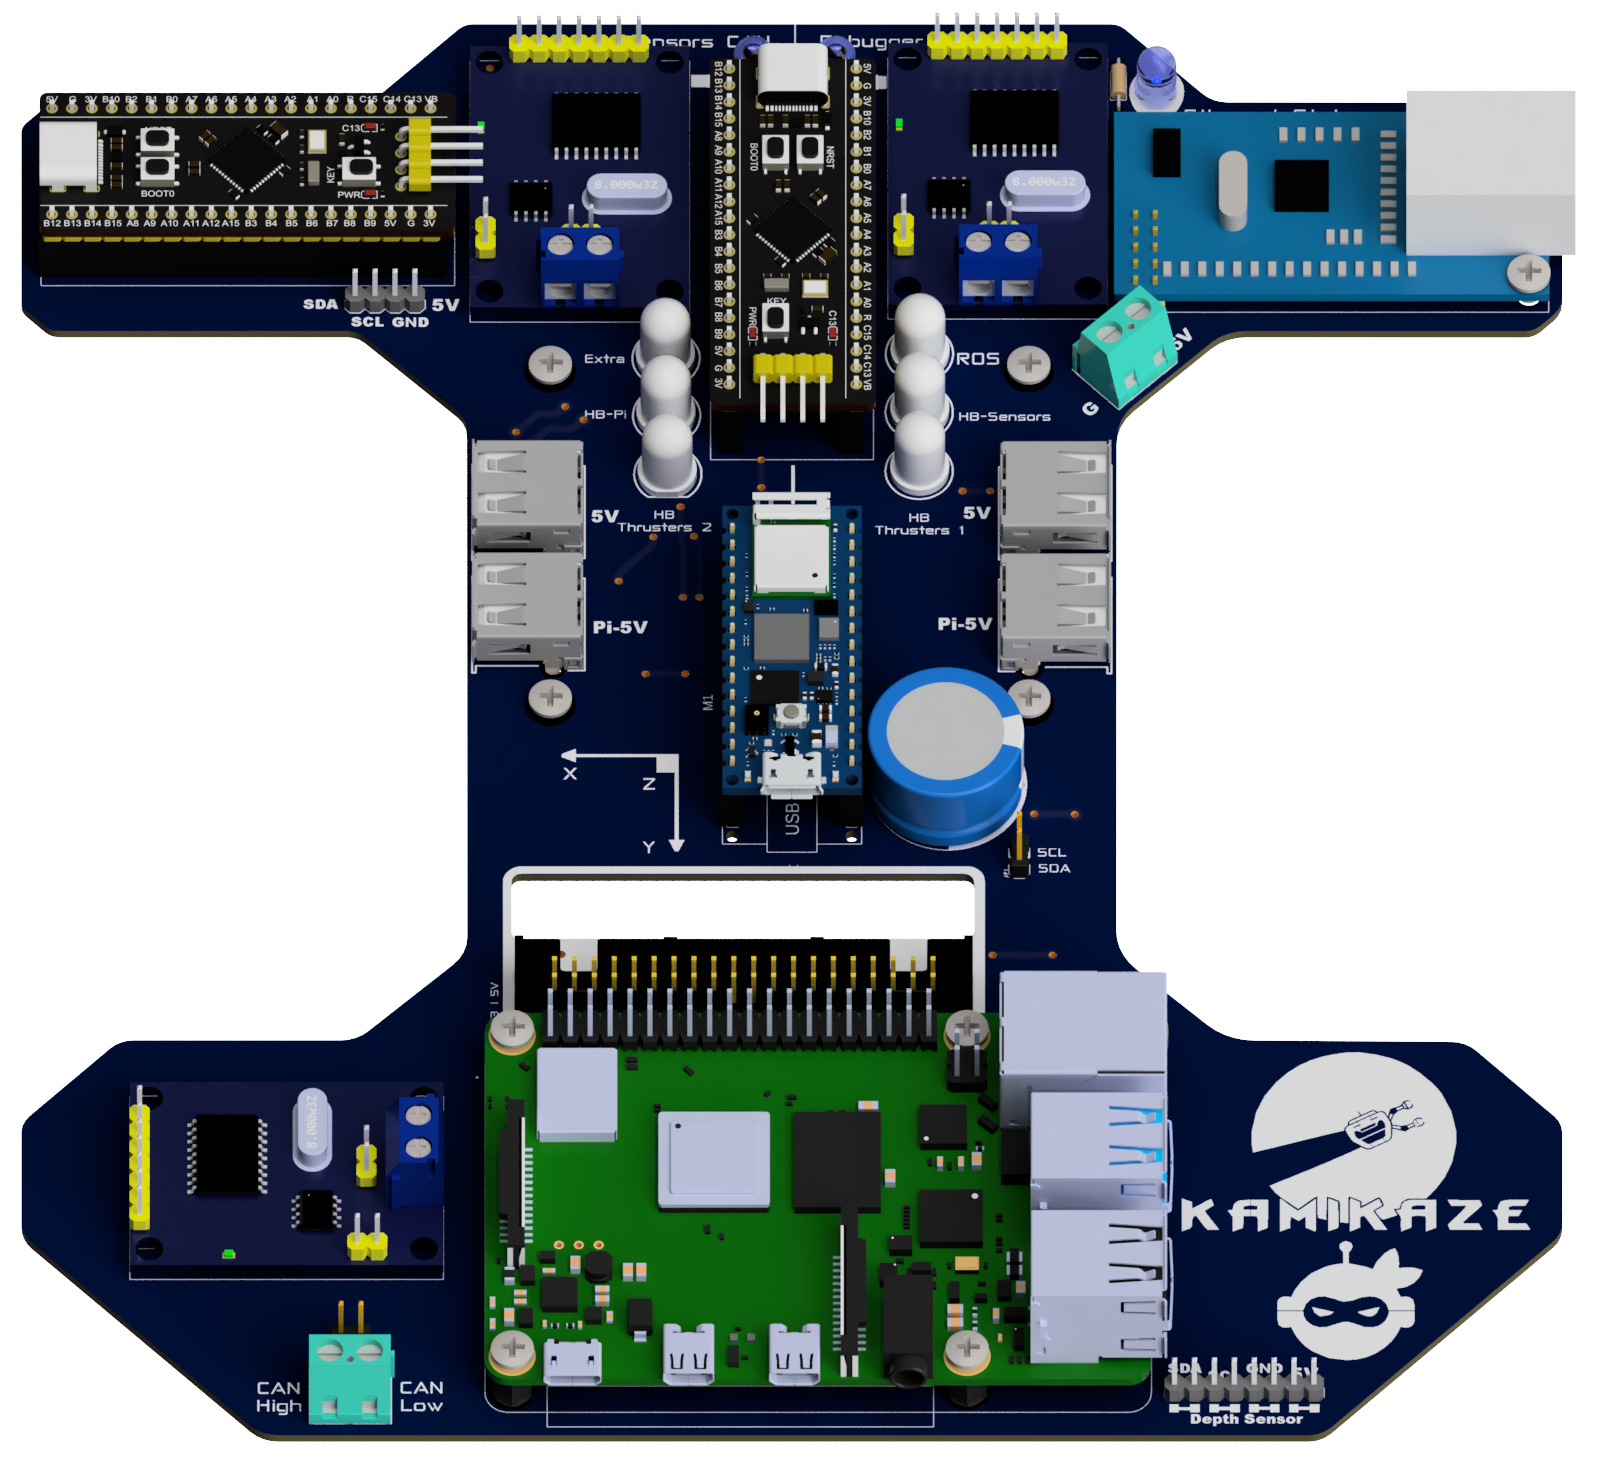
\includegraphics[width=\textwidth]{Sections/2Design Rationale/images/Control PCB.png}
      \caption{Control PCB.}
    \end{subfigure}
  
    \vspace{10pt}
    \begin{subfigure}{0.8\columnwidth}
      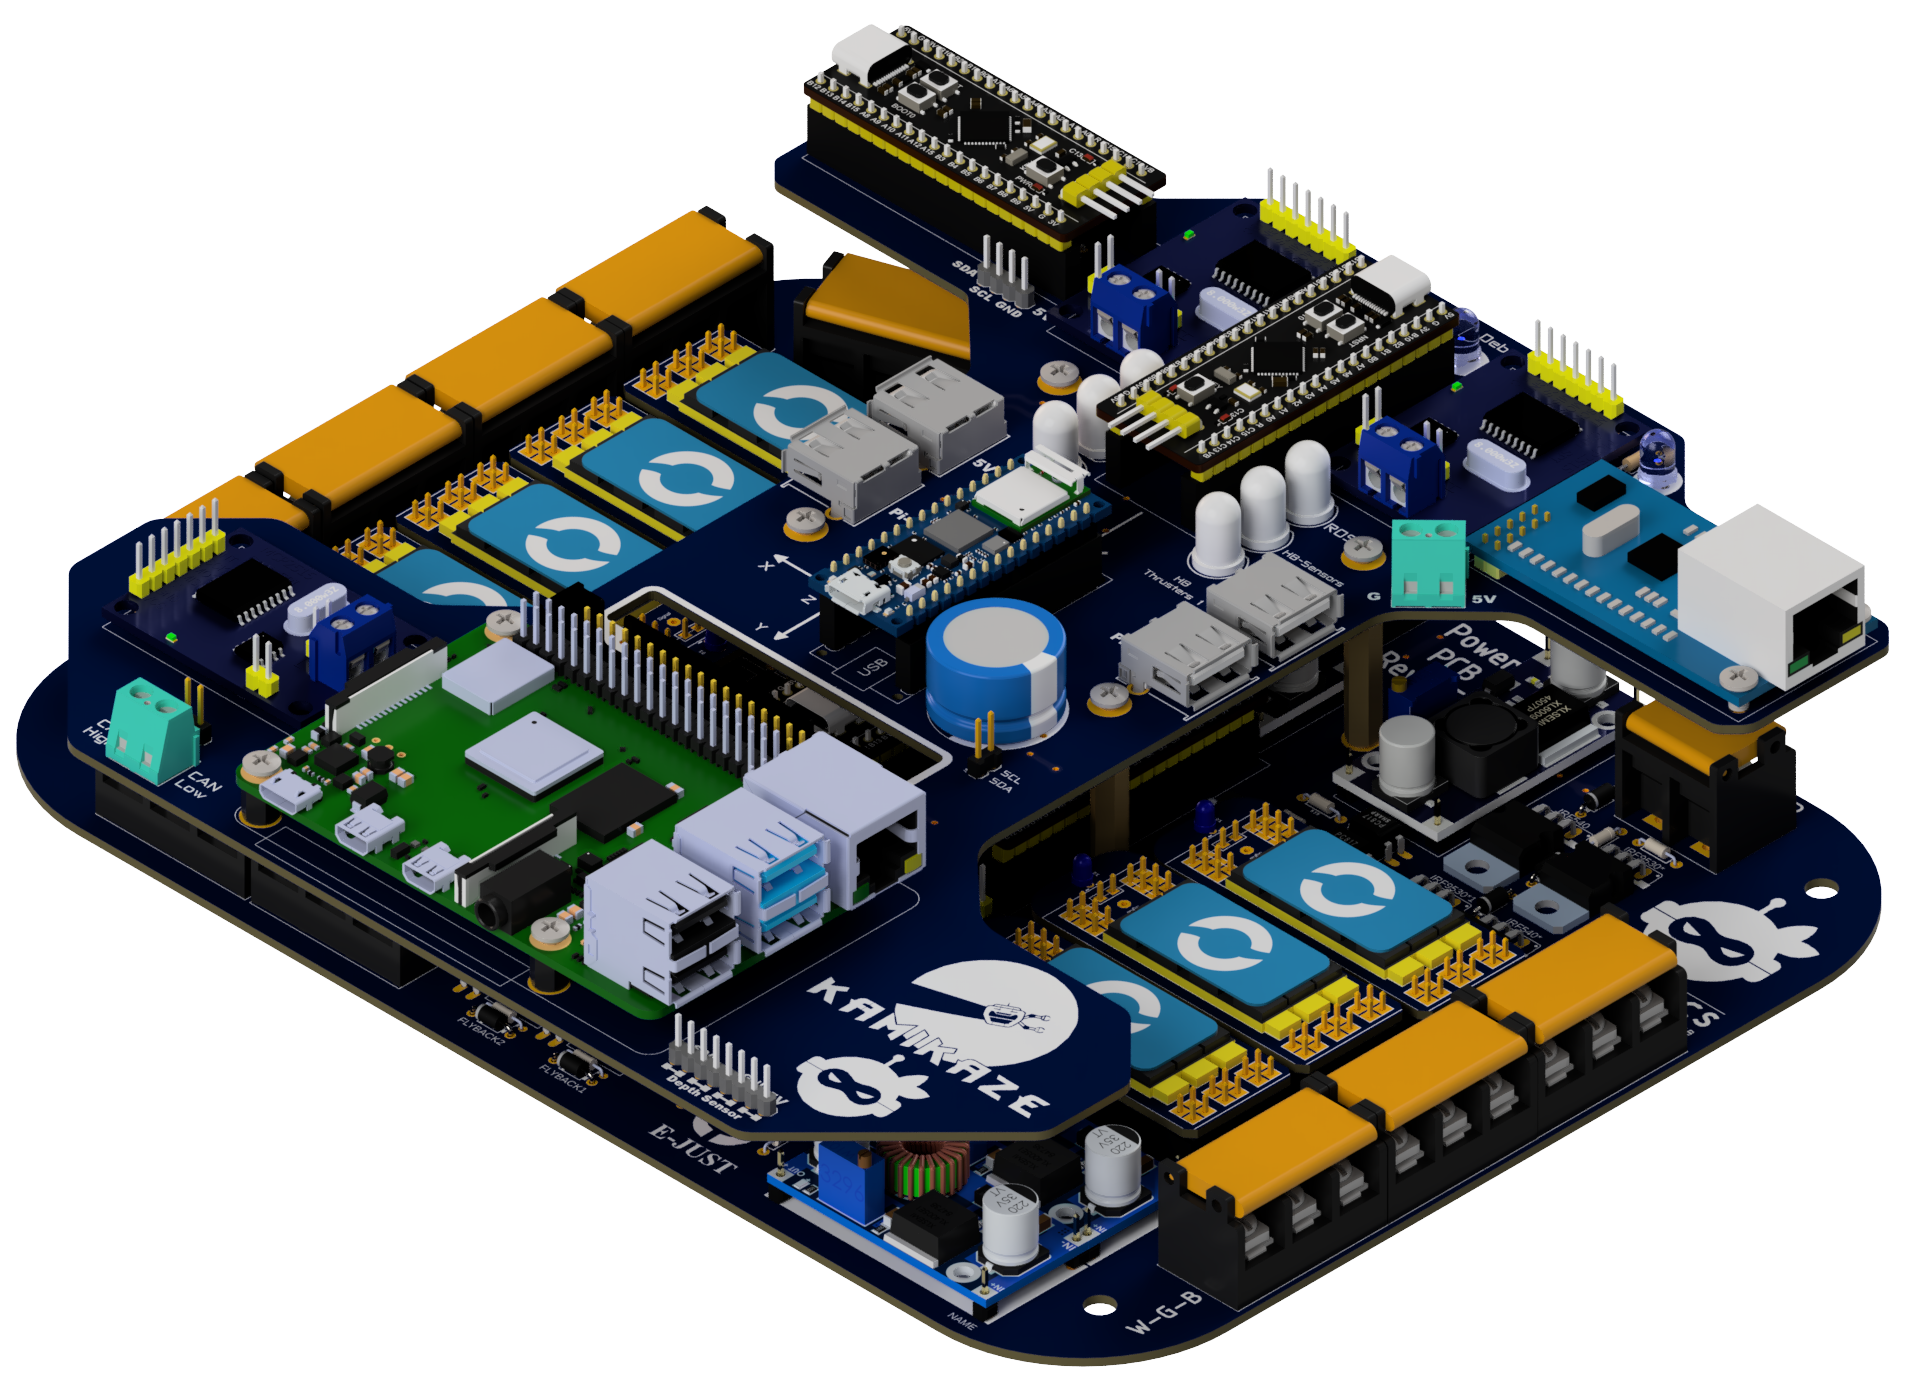
\includegraphics[width=\textwidth]{Sections/2Design Rationale/images/Full Stack.png}
      \caption{Full stack of PCBs.}
    \end{subfigure}
    \caption{Kamikaze PCBs.}
    \label{fig:pcb}
  \end{figure}

Finally, the complete ROV assembly was tested to ensure seamless integration of mechanical, electrical, and software components.